\documentclass[tikz,border=3.14mm]{standalone}
\usepackage{pgfplots}
\pgfplotsset{compat=1.17}
\usepackage{glossaries} % For \gls{pcnc}

\begin{document}
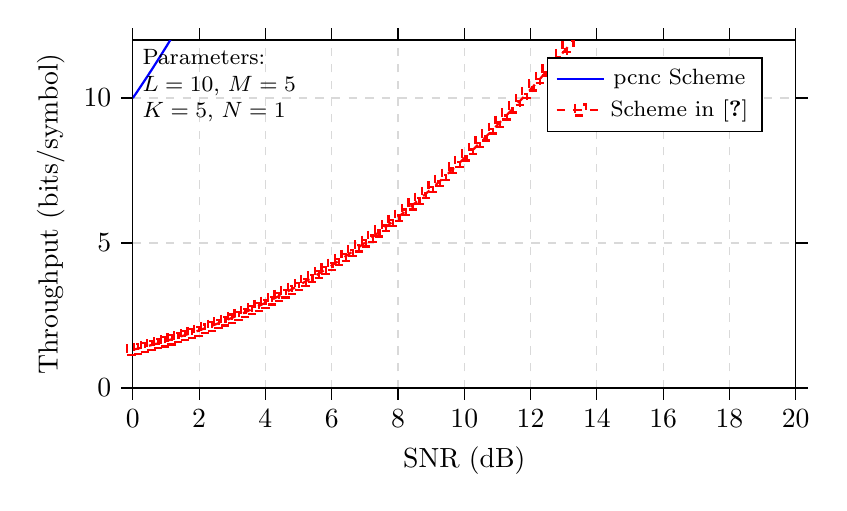
\begin{tikzpicture}
  \begin{axis}[
    width=10cm,
    height=6cm,
    xlabel={SNR (dB)},
    ylabel={Throughput (bits/symbol)},
    xmin=0, xmax=20,
    ymin=0, ymax=12,
    grid=both,
    grid style={dashed, gray!30},
    legend style={at={(0.95,0.95)}, anchor=north east, font=\footnotesize},
    tick align=outside,
    tick style={black, thin}
  ]
    
    % PCNC Scheme (Assumed convex curve)
    \addplot[
      color=blue,
      mark=none,
      thick,
      domain=0:20,
      samples=100
    ] {10 * log2(1 + 10^(x/10))}; % L=10, N=1
    \addlegendentry{\gls{pcnc} Scheme}
    
    % Reference Scheme (Antonioli 2023)
    \addplot[
      color=red,
      mark=square,
      dashed,
      thick,
      domain=0:20,
      samples=100
    ] {5 * log2(1 + 10^(x/10)/5)}; % M=5, K=5
    \addlegendentry{Scheme in~\cite{antonioli2023mixed}}
    
    % Annotate parameters (placed at upper left)
    \node[anchor=north west, font=\footnotesize, align=left] at (axis cs:0,12) {
      Parameters:\\
      $L=10$, $M=5$\\
      $K=5$, $N=1$
    };
  \end{axis}
\end{tikzpicture}
\end{document}